\documentclass[
  % all of the below options are optional and can be left out
  % course name (default: 2IL50 Data Structures)
  course = {{16-811 Math Fundamentals for Robotics}},
  % quartile (default: 3)
  quartile = {{1}},
  % assignment number/name (default: 1)
  assignment = 3,
  % student name (default: Some One)
  name = {{Kangle Deng}},
  % student number, NOT S-number (default: 0123456)
  % studentnumber = {{0123456 ; 0314159}},
  % student email (default: s.one@student.tue.nl)
  email = {{kangled@andrew.cmu.edu}},
  % first exercise number (default: 1)
  firstexercise = 1
]{aga-homework}


\begin{document}

\exercise
\subexercise
\begin{equation*}
    f(x) = -0.5 + x - \frac{1}{3}x^3 + \frac{1}{5!}x^5 + \cdots + (-1)^{k+1}\frac{1}{k!}x^k + \cdots, \qquad k = 1,2,3,\cdots
\end{equation*}

\subexercise

Fig \ref{fig:hw3_ex1b} is the result.

\begin{figure}
    \centering
    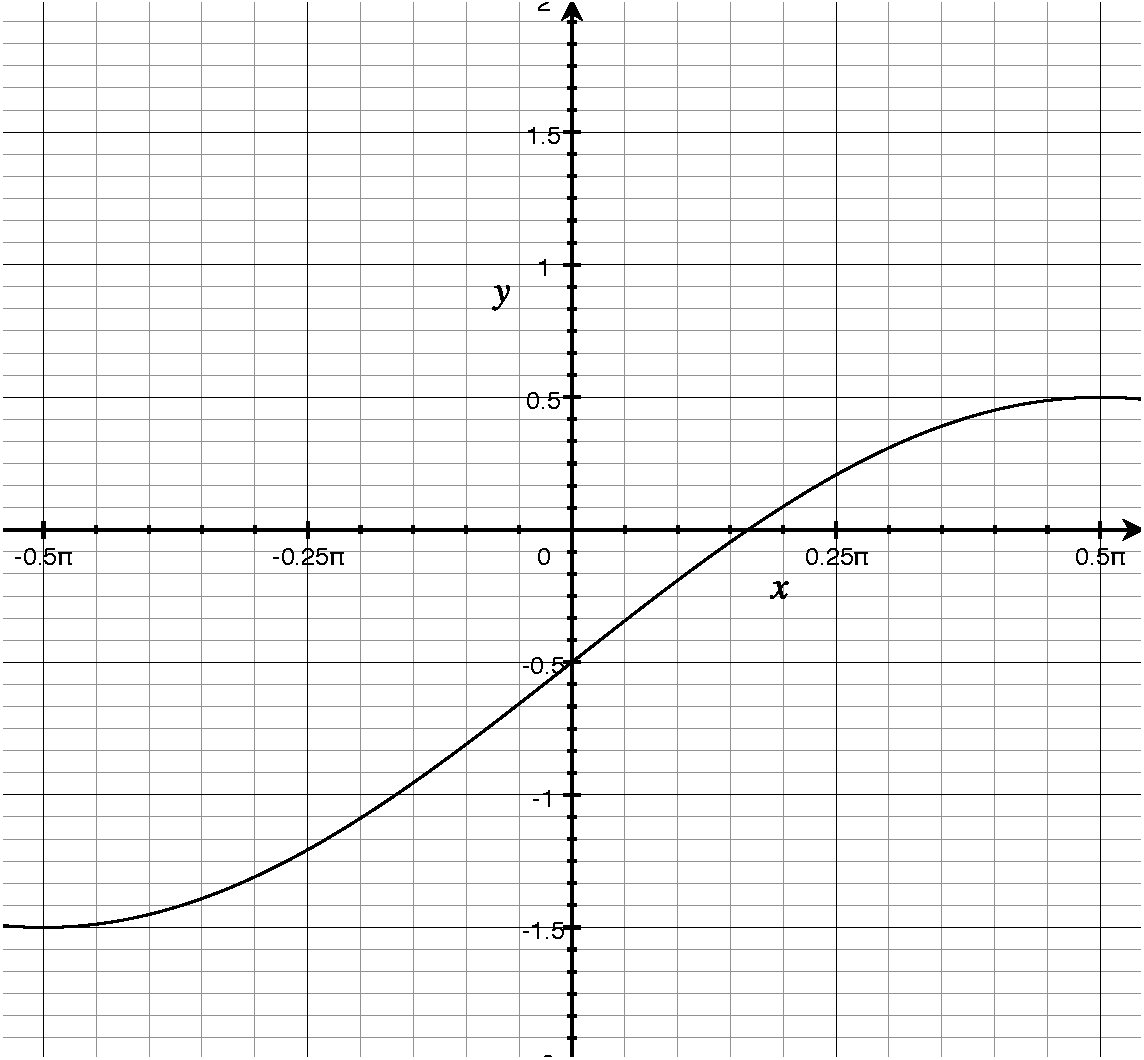
\includegraphics[width = .6\textwidth]{math/fig/hw3/ex1b.pdf}
    \caption{Ex1(b) $f(x) = \sin x - 0.5$.}
    \label{fig:hw3_ex1b}
\end{figure}

\subexercise
First calculate the best uniform approximation by a linear function. Then prove that is also the best uniform approximation of degree 2. Let $p(x) = bx + c$.

From the odd symmetry regarding y-axis, we derive that $c = -0.5$. Otherwise, one can always decrease the $L_{\infty}$ by setting $c$ as $-0.5$.

By examining the graph of $f(x)$, it looks plausible that a good linear approximation $p(x)$ would overestimates $f(x)$ at $x = \frac{\pi}{2}$ and a point $x_1$ near $x = -\frac{\pi}{4}$, and most underestimates $f(x)$ at $x = -\frac{\pi}{2}$ and and a point $-x1$ near $x = \frac{\pi}{4}$. Let $E$ be the maximum error. We have:

\begin{equation*}
    \begin{aligned}
    \sin(-\frac{\pi}{2}) + b \cdot \frac{\pi}{2} & = E, \\
    \sin(x_1) - b x_1 & = -E.
    \end{aligned}
\end{equation*}

So,
\begin{equation*}
    -1 + b \cdot (\frac{\pi}{2} - x) + \sin(x_1) = 0.
\end{equation*}

Let $e(x) = f(x) - p(x) = \sin(x) - bx$. Then $e(x)$ should reach local minimum at $x = x_1$. This implies $e'(x_1) = \cos(x_1) - b = 0$. Then we have $b = \cos(x_1)$. So:

\begin{equation*}
    -1 + \cos(x_1) \cdot (\frac{\pi}{2} - x) + \sin(x_1) = 0.
\end{equation*}

I use a predefined routine $scipy.optimize.fsolve$ to solve this equation near $x = -\frac{\pi}{4}$, and get:

\begin{equation*}
    \begin{aligned}
     x_1 & = -0.7603, \\
     b & = \cos(x_1) = 0.7246, \\
     E & = -1 + b \cdot \frac{\pi}{2} = 0.1382.
    \end{aligned}
\end{equation*}

Note that $e(x)$ reaches its local maximum and local minimum at $x = -\frac{\pi}{2}, -0.7603, 0.7603, \frac{\pi}{2}$, the alternating set has length 5. So $p(x) = 0.7246x-0.5$ is also the quadratic best uniform approximation.

From the analysis above, we have $L_{\infty} = E = 0.1382$. And, 

\begin{equation*}
\begin{aligned}
    L_2 & = \sqrt{\int_{-\frac{\pi}{2}}^{\frac{\pi}{2}}|\sin(x)-bx|^2dx} = \sqrt{\int_{-\frac{\pi}{2}}^{\frac{\pi}{2}}(\sin^2(x) + b^2x^2 - 2bx\sin(x))dx} \\
    & = \sqrt{\int_{-\frac{\pi}{2}}^{\frac{\pi}{2}}\sin^2(x)dx + b^2\int_{-\frac{\pi}{2}}^{\frac{\pi}{2}}x^2 dx - 2b\int_{-\frac{\pi}{2}}^{\frac{\pi}{2}} x\sin(x)dx}.
\end{aligned}
\end{equation*}

Note that
\begin{equation*}
    \begin{aligned}
        & \int_{-\frac{\pi}{2}}^{\frac{\pi}{2}}\sin^2(x)dx = \frac{1}{2}\int_{-\frac{\pi}{2}}^{\frac{\pi}{2}} (1 - \cos(2x))dx = \frac{\pi}{2} - \frac{1}{2}\int_{-\frac{\pi}{2}}^{\frac{\pi}{2}} \cos(2x) dx = \frac{\pi}{2},\\
        & \int_{-\frac{\pi}{2}}^{\frac{\pi}{2}}x^2 dx = \frac{1}{3} \cdot \frac{\pi^3}{4} = \frac{\pi^3}{12},\\
        & \int_{-\frac{\pi}{2}}^{\frac{\pi}{2}} x\sin(x)dx  = -\int_{-\frac{\pi}{2}}^{\frac{\pi}{2}} x d\cos(x) = \int_{-\frac{\pi}{2}}^{\frac{\pi}{2}} \cos(x)dx = 2.
    \end{aligned}
\end{equation*}

So, 
\begin{equation*}
    L_2 = \sqrt{\frac{\pi}{2} + b^2 \cdot \frac{\pi^3}{12} - 4b} = 0.1704.
\end{equation*}

\subexercise
Suppose the inner product is given by the rule $<g,h> = \int_{-\frac{\pi}{2}}^{\frac{\pi}{2}}g(x)h(x)dx$.

First construct the orthogonal sequence of polynomials using the recurrence relation.
\begin{itemize}
    \item Define $p_0(x) = 1.$ So $<p_0,p_0> = \pi, <xp_0, p_0> = 0$.
    \item $p_1(x) = (x-0)p_0(x) = x.$ So $<p_1, p_1> = \frac{\pi^3}{12}, <xp_1, p_1> = 0$.
    \item $p_2(x) = (x-0)p_1(x) - \frac{\pi^2}{12}p_0(x) = x^2 - \frac{\pi^2}{12}$.
\end{itemize}

Then we compute:
\begin{equation*}
    \begin{aligned}
        <f, p_0> & = \int_{-\frac{\pi}{2}}^{\frac{\pi}{2}}(\sin(x) - 0.5)dx = -\frac{\pi}{2}, \\
        <f, p_1> & = \int_{-\frac{\pi}{2}}^{\frac{\pi}{2}}(\sin(x) - 0.5)xdx = 2, \\
        <f, p_2> & = \int_{-\frac{\pi}{2}}^{\frac{\pi}{2}}(\sin(x) - 0.5)(x^2-\frac{\pi^2}{12})dx = 0.
    \end{aligned}
\end{equation*}

So we have $\hat{p}(x) = \sum \limits_{i=0}^2 \frac{<f,p_i>}{<p_i,p_i>}p_i(x) = \frac{24}{\pi^3}x - 0.5 = 0.7740x - 0.5$.

\begin{equation*}
    L_2 = \sqrt{\frac{\pi}{2} + b^2 \cdot \frac{\pi^3}{12} - 4b} = 0.1507.
\end{equation*}

To calculate $L_{\infty}$, we have $e(x) = \sin(x) - bx$. When $e'(x) = 0$, $x = \cos^{-1}b = 0.6856$. Then we calculate $e(0.6856) = 0.1025, e(\frac{\pi}{2}) = -0.2159$. So $L_\infty = 0.2159$.

\exercise
The visualization of the data points is shown in Figure \ref{fig:hw3_ex2}. By checking the figure, we can see the periodic phenomenon that $[0,1]$ interval contains $2.5$ ``periods''. We can also see the global trend is like a linear function. So we assume $f(x) = a + bx + c\sin(5\pi x)$.

\begin{figure}
    \centering
    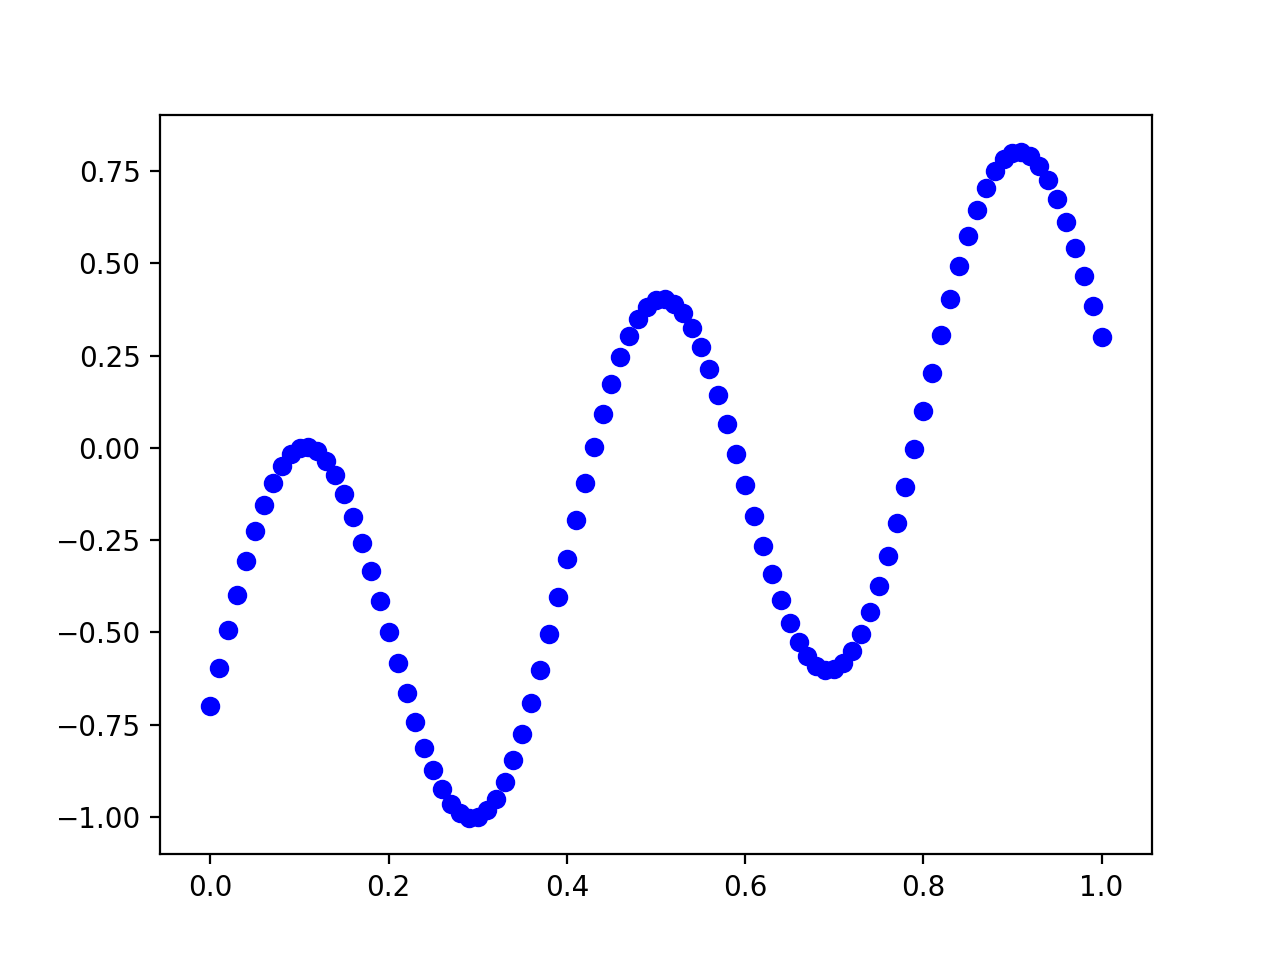
\includegraphics{math/fig/hw3/ex2.png}
    \caption{Ex2: Visualization of data points}
    \label{fig:hw3_ex2}
\end{figure}

To find $a,b,c$, we have the following equations:

\begin{equation*}
    \left(
    \begin{array}{ccc}
        1 & 0 & \sin(5\pi \cdot 0) \\
        1 & 1/100 & \sin(5\pi \cdot 1/100) \\
        \cdots & \cdots & \cdots \\
        1 & 1 & \sin(5\pi \cdot 1) \\
    \end{array}
    \right)_{101 \times 3} \cdot
    \left(
    \begin{array}{c}
        a \\ b \\ c
    \end{array}
    \right)
     = f_{101 \times 1}
\end{equation*}
where $f$ is the data vector.

Since this is an over-constrained system, we can solve it by SVD decomposition (I implement it in $ex2.py$), and get the answer: $a = -0.7, b = 1, c=0.6$. Therefore, $f(x) = -0.7 + x + 0.6\sin(5\pi x)$. And $L_2 = 5.59e-15$.

\exercise
\subexercise
\begin{equation*}
    \begin{aligned}
        T_0(x) &= 1, \\
        T_1(x) &= x, \\
        T_2(x) &= 2xT_1(x) - T_0(x) = 2x^2 - 1, \\
        T_3(x) &= 2xT_2(x) - T_1(x) = 2x(2x^2-1) - x = 4x^3 - 3x,\\
        T_4(x) &= 2xT_3(x) - T_2(x) = 2x(4x^3 - 3x) - (2x^2 - 1) = 8x^4 - 8x^2 + 1, \\
        T_5(x) &= 2xT_4(x) - T_3(x) = 2x(8x^4 - 8x^2 + 1) - (4x^3 - 3x) = 16x^5 - 20x^3 + 5x.
    \end{aligned}
\end{equation*}

\subexercise
Note that $(1-x^2)^{-1/2}$ is an even function over $[-1,1]$, so we only need to show that $T_4(x)T_5(x)$ is an odd function over $[-1,1]$. This is easy to show because $T_4(x)$ is an even function while $T_5(x)$ is an odd function over $[-1,1]$.

Therefore, $(1-x^2)^{-1/2}T_4(x)T_5(x)$ is an odd function over $[-1,1]$, which means $\int_{-1}^1(1-x^2)^{-1/2}T_4(x)T_5(x)dx=0$.

\subexercise
\begin{equation*}
    \begin{aligned}
        <T_n,T_n> & = \int_{-1}^1(1-x^2)^{-1/2}T_n(x)T_n(x)dx \\
        & = \int_{-1}^1(1-\cos^2 \theta)^{-1/2}T_n(\cos \theta)T_n(\cos \theta)d\cos \theta \\
        & = \int_{\pi}^0(1-\cos^2 \theta)^{-1/2}\cos (n\theta)\cos (n\theta)(-\sin \theta) d\theta \\
        & = \int_{0}^{\pi}(\sin^2 \theta)^{-1/2}\cos (n\theta)\cos (n\theta)\sin \theta d\theta \\
        & = \int_{0}^{\pi}\cos^2 (n\theta) d\theta \\
        & = \frac{1}{2} \int_{0}^{\pi}(\cos (2n\theta) + 1) d\theta \\
        & = \frac{1}{2} (\int_{0}^{\pi}\cos (2n\theta)d \theta + \int_{0}^{\pi}1 d \theta)  \\
        & = \frac{1}{2} (0 + \pi)  \\
        & = \frac{\pi}{2}.
    \end{aligned}
\end{equation*}

Therefore, the length of $T_n$ is $\sqrt{\frac{\pi}{2}}$.

\subexercise
\begin{equation*}
    \begin{aligned}
        <T_i,T_j> & = \int_{-1}^1(1-x^2)^{-1/2}T_i(x)T_j(x)dx \\
        & = \int_{-1}^1(1-\cos^2 \theta)^{-1/2}T_i(\cos \theta)T_j(\cos \theta)d\cos \theta \\
        & = \int_{\pi}^0(1-\cos^2 \theta)^{-1/2}\cos(i \theta)\cos(j \theta) (-\sin \theta) d \theta \\
        & = \int_{0}^{\pi}(\sin^2 \theta)^{-1/2}\cos(i \theta)\cos(j \theta) \sin \theta d \theta \\
        & = \int_{0}^{\pi}\cos(i \theta)\cos(j \theta)d \theta \\
        & = \frac{1}{2}\int_{0}^{\pi}(cos((i+j)\theta) + cos((i-j)\theta))d \theta \\
        & (\text{Note that $\int_{0}^{\pi}cos(k\theta)d\theta = 0, k \in \mathbb{Z}$ and $k \ne 0$.}) \\
        & = 0. \qquad \text{(Because $i \ne j$.)}
    \end{aligned}
\end{equation*}

\exercise
\subexercise
Suppose a plane is defined by: $ax + by + cz = 1$. Our goal is to solve the minimize problem $\min \limits_{a,b,c} \sum \limits_{i=1}^n (ax_i + by_i + cz_i - 1)^2$.

Let
\begin{equation*}
    P = \left(
    \begin{array}{ccc}
        x_1 & y_1 & z_1 \\
        x_2 & y_2 & z_2 \\
        \cdots & \cdots & \cdots \\
        x_n & y_n & z_n \\
    \end{array}
    \right)_{n \times 3}
\end{equation*}
and $\alpha = (a,b,c)^T$. Then the minimize problem can be written as:

\begin{equation*}
    \min_{\alpha} ||P\alpha - 1_{n \times 1} ||^2.
\end{equation*}

From the previous lecture on SVD, this problem is equivalent to get the SVD solution of the linear equation $P\alpha = 1_{n \times 1}$.

Therefore, $\alpha = (P^TP)^{-1}P^T\cdot 1_{n \times 1} = (0.19264892, 2.01385644, 0.09978737)^T$. So the plane is $0.19264892x + 2.01385644y + 0.09978737z = 1$. The average distance is $\frac{1}{n} \sum \limits_{i=1}^n \frac{|ax_i+by_i+cz_i-1|}{\sqrt{a^2+b^2+c^2}} = 0.00274$.

Fig \ref{fig:hw3_ex4a} is the visualization.

\begin{figure}
    \centering
    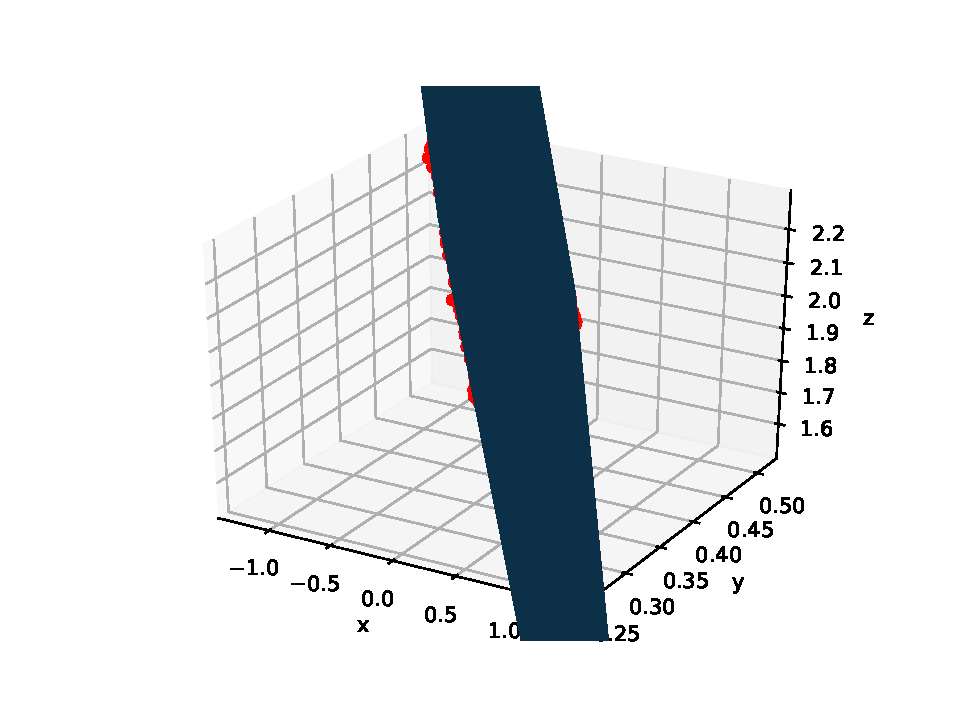
\includegraphics{math/fig/hw3/ex4a.pdf}
    \caption{Ex4(a) Fitted plane and data points.}
    \label{fig:hw3_ex4a}
\end{figure}

\subexercise

Fig \ref{fig:hw3_ex4b} is the visualization. The fitted plane is not close to the actual table, and tilts to the clutter. Because the least square solution considers all of the data including those outliers that should not be considered.

%alpha: [0.12602863 1.25698279 0.2698782 ]

\begin{figure}
    \centering
    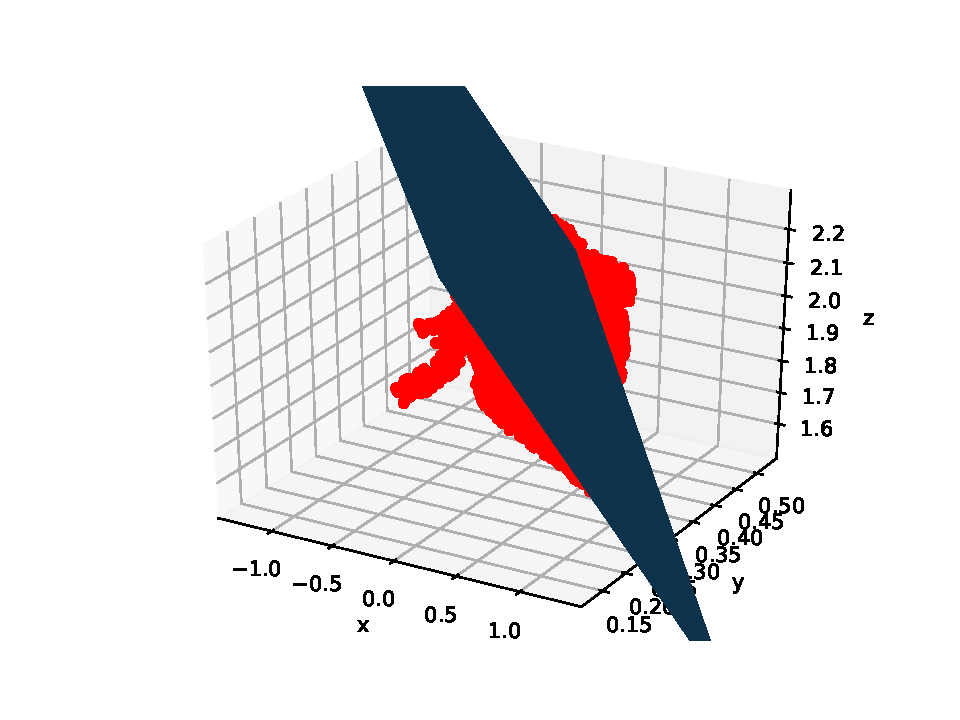
\includegraphics{math/fig/hw3/ex4b.pdf}
    \caption{Ex4(b) Fitted plane and data points.}
    \label{fig:hw3_ex4b}
\end{figure}

\subexercise

I use RANSAC algorithm to prevent the effect of outliers. The steps are as follow:

\begin{itemize}
    \item Randomly choose $N$ points from the data, and fit a plane with them.
    \item Check the number of points whose distance from that fitted plane is less than $ERROR$. Suppose that number is $t$.
    \item If $t$ is bigger than a threshold (a proportion $k$ of the number of all the points), then use these $t$ points to fit a new plane and output. Otherwise, repeat the previous 2 steps until reaching maximum iterations.
\end{itemize}

Specifically in this problem, I set $N$ as $100$, $ERROR$ as $0.01$, and $k$ as $0.8$. Fig \ref{fig:hw3_ex4c} is the visualization. $\alpha = (0.20446216,2.01896897,0.09829537)^T$, which is close to the result in Ex4(a). I implement this as a function $RANSAC()$ in $ex4.py$.

\begin{figure}
    \centering
    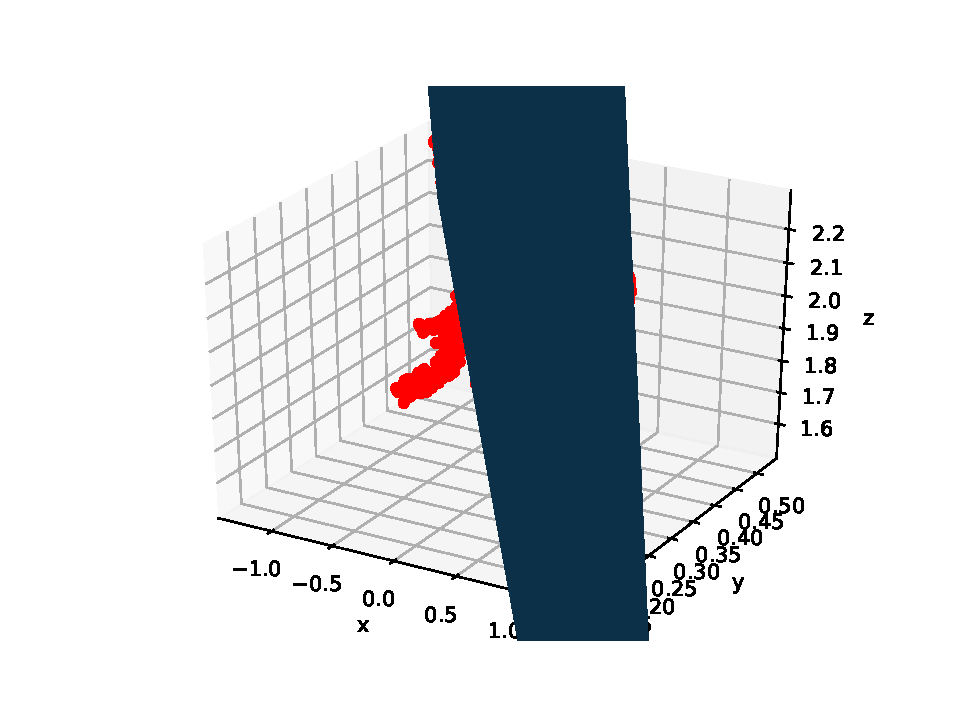
\includegraphics{math/fig/hw3/ex4c.pdf}
    \caption{Ex4(c) Fitted plane and data points.}
    \label{fig:hw3_ex4c}
\end{figure}

\subexercise
The algorithm is as follow:
\begin{itemize}
    \item Randomly choose $N$ points from the data, and fit a plane with them.
    \item Check the number of points whose distance from that fitted plane is less than $ERROR$. Suppose that number is $t$.
    \item If $t$ is bigger than a threshold (a proportion $k$ of the number of all the points), then use these $t$ points to fit a new plane and add it to the plane list. Then remove those $t$ points from the data. If $t$ is smaller than the threshold, repeat the previous 2 steps until reaching maximum iterations.
    \item Stop searching when already having 4 planes.
\end{itemize}

Specifically in this problem, I set $N$ as $5$, $ERROR$ as $0.01$, and $k$ as $0.15$. Fig \ref{fig:hw3_ex4d} is the visualization. $\alpha_1 = (-0.7945602,   4.62651056,  0.18415421)^T,\alpha_2 = (-0.09322498,  0.54385651,  0.02086644)^T,\alpha_3=(0.53226005,  0.09583805, -0.11503434)^T,\alpha_4 = (4.44086799,  0.77447499, -0.90945754)^T$, which is close to the result in Ex4(a). I implement this in $ex4d.py$.

\begin{figure}
    \centering
    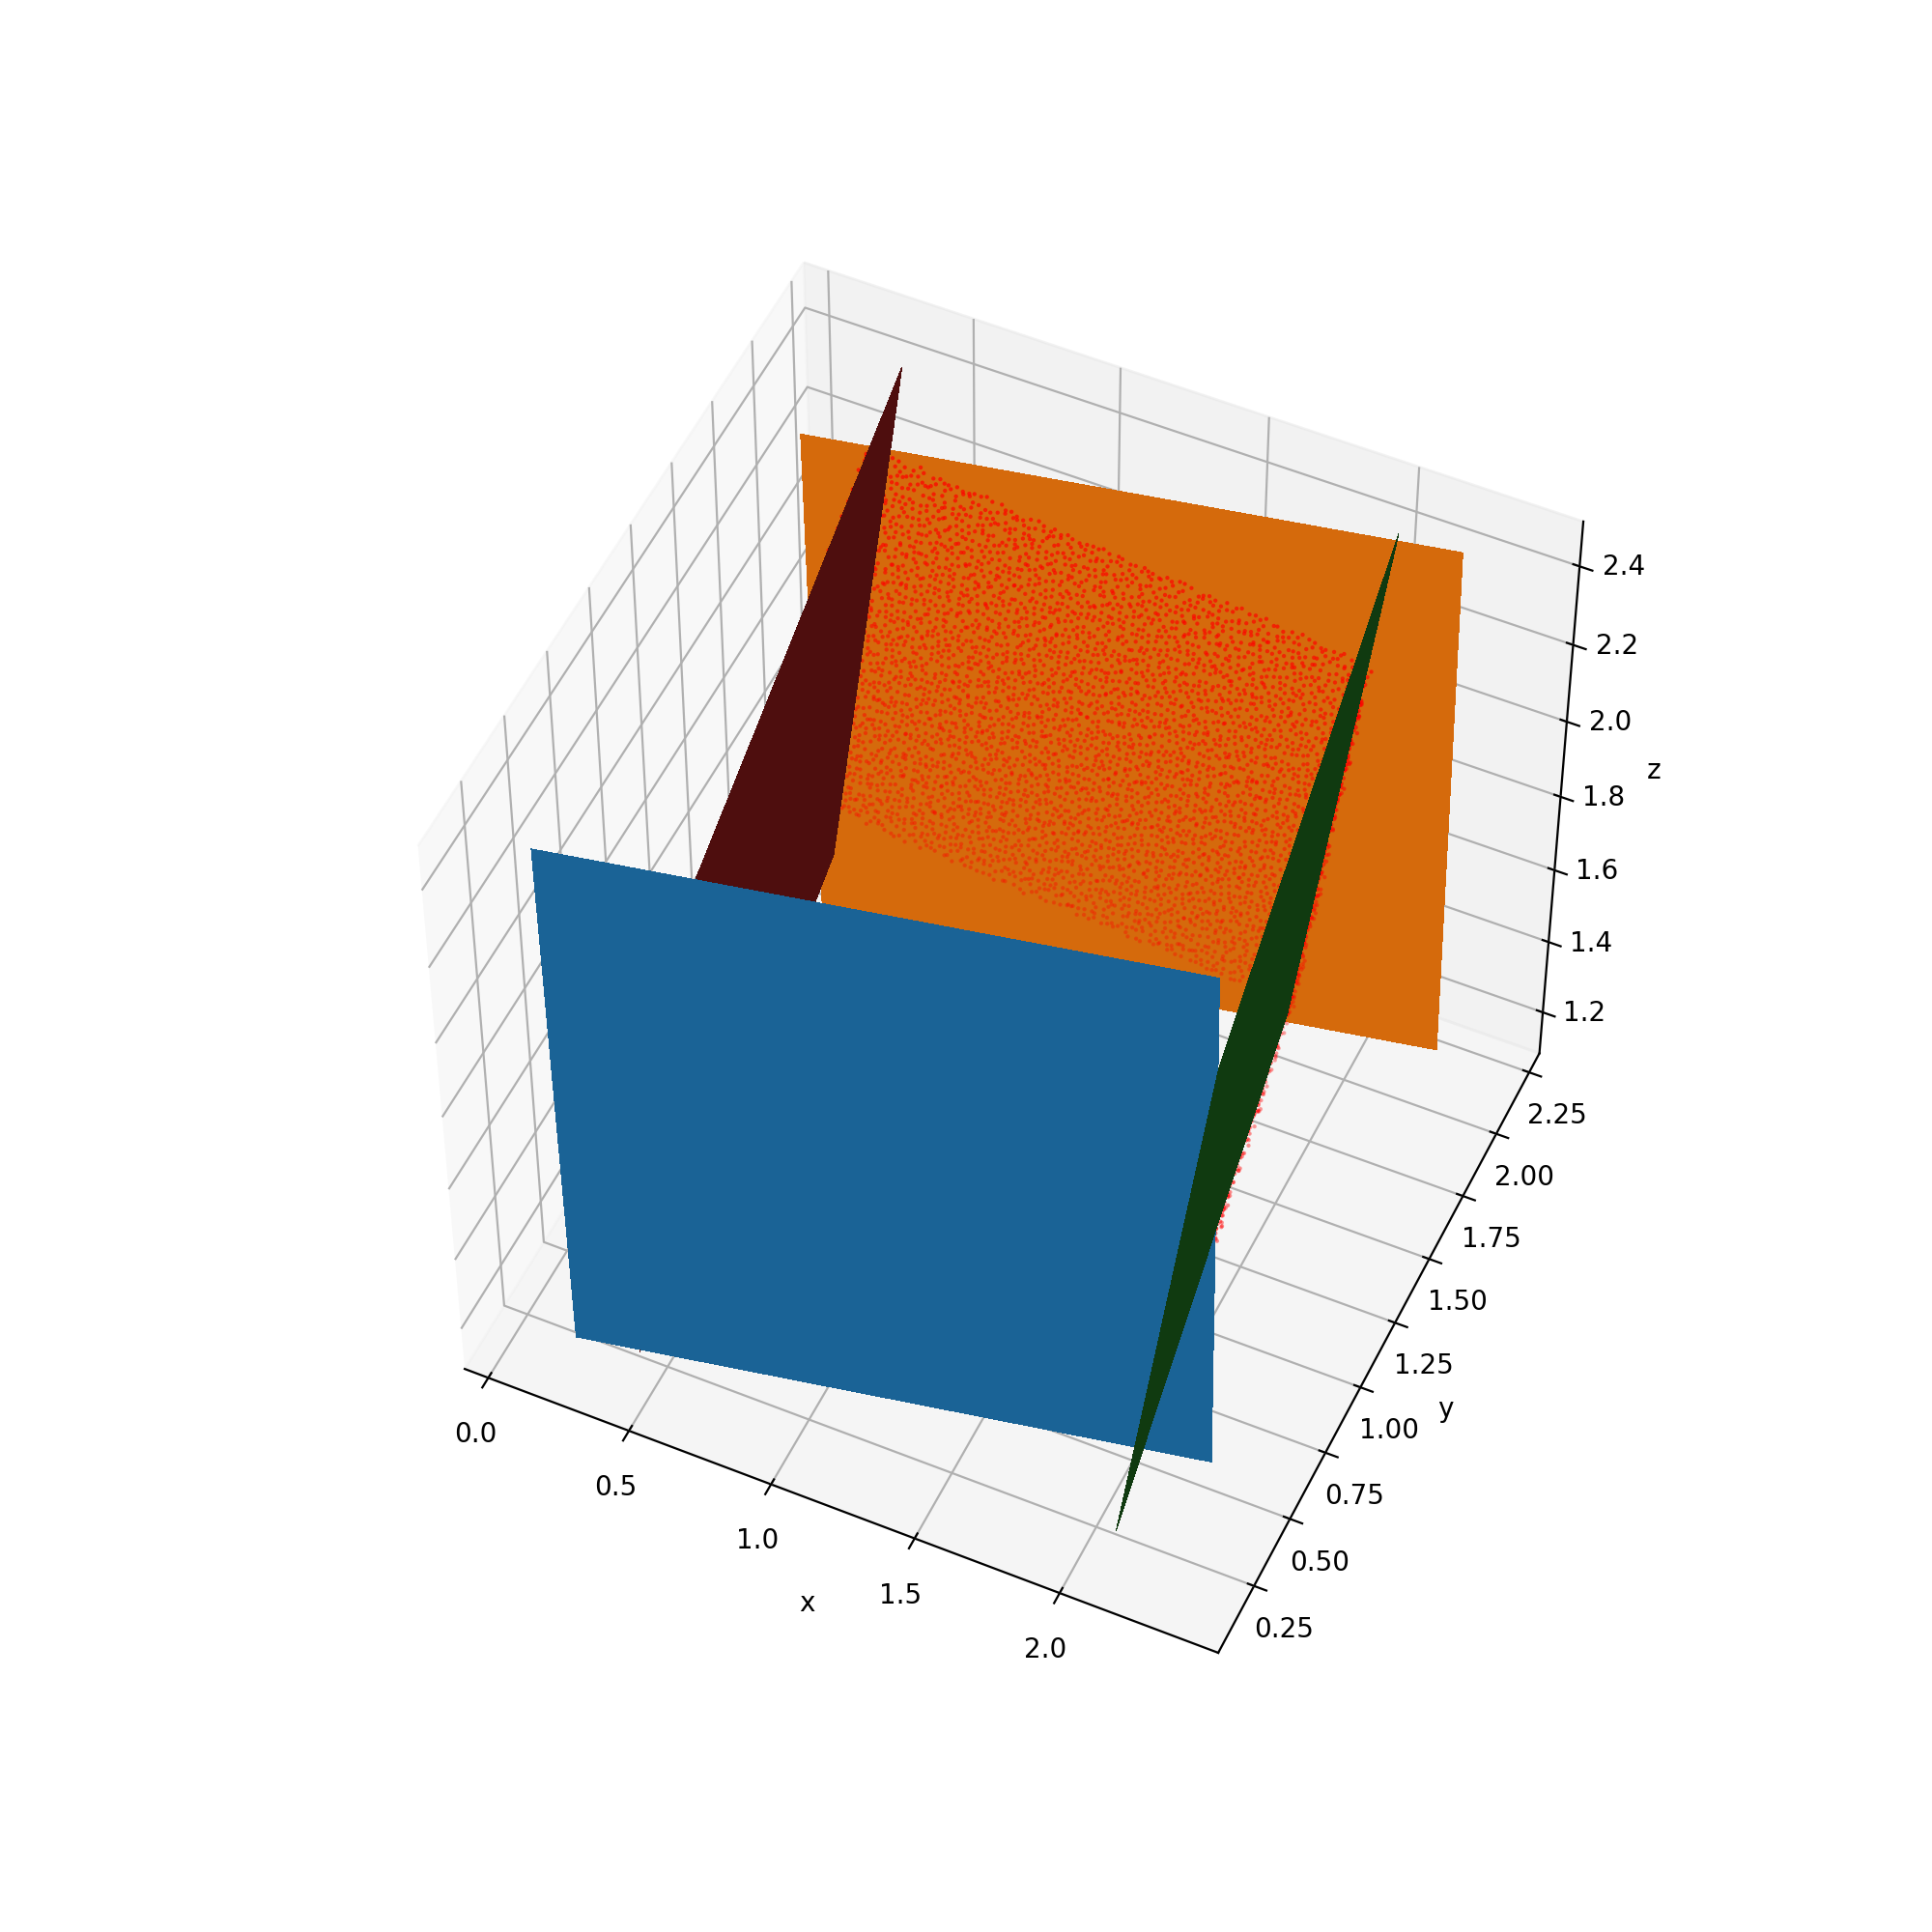
\includegraphics[width=\textwidth]{math/fig/hw3/ex4d.png}
    \caption{Ex4(d) Fitted plane and data points.}
    \label{fig:hw3_ex4d}
\end{figure}

\subexercise
I refine the algorithm in 4(d). 
\begin{itemize}
    \item In order to find the plane with not so many points, I use a progressive decaying $k$. Once a round of searching fails (reaching maximum iterations), I divide the threshold $k$ by 2 to search for the planes with less points.
    \item To avoid extracting similar planes, when finding a plane during searching, I compare it to those already found planes. If this is too similar to the found ones, the algorithm drops it and keeps searching for another one.
\end{itemize}

I set the maximum iterations as 100000, and the initial $k$ as 0.2. I implement this in $ex4e.py$.

To calculate the smoothness score of the planes, for each plane $p$, I first identify those data points near $p$ (distance less than 0.01). And use those $m$ points to calculate the standard deviation of the directional distances:

\begin{equation*}
    \sqrt{\frac{1}{m}\sum \limits_{i=0}^m (\frac{ax_i+by_i+cz_i-1}{\sqrt{a^2+b^2+c^2}} - \frac{1}{m} \sum \limits_{j=0}^m \frac{ax_j+by_j+cz_j-1}{\sqrt{a^2+b^2+c^2}})^2}
\end{equation*}

Those four planes and the smoothness scores are as follow:
\begin{equation*}
    \begin{aligned}
        \alpha_1 & = (0.02218274,1.70745748,-0.17411718)^T, & s_1 = 0.0054122\\
        \alpha_2 & = (-0.03004499, -1.8524345,   0.17541391)^T, & s_2 = 0.0048909\\
        \alpha_3 & = (1.3488192,  -0.02666764, -0.08425115)^T, & s_3 = 0.0057762 \\
        \alpha_4 & = (-1.05988179, -0.07900652, -0.08789204)^T, & s_4 = 0.0058500\\
    \end{aligned}
\end{equation*}

So the smoothest plane is $\alpha_2$, which is the blue plane in Figure \ref{fig:hw3_ex4e}.

\begin{figure}
    \centering
    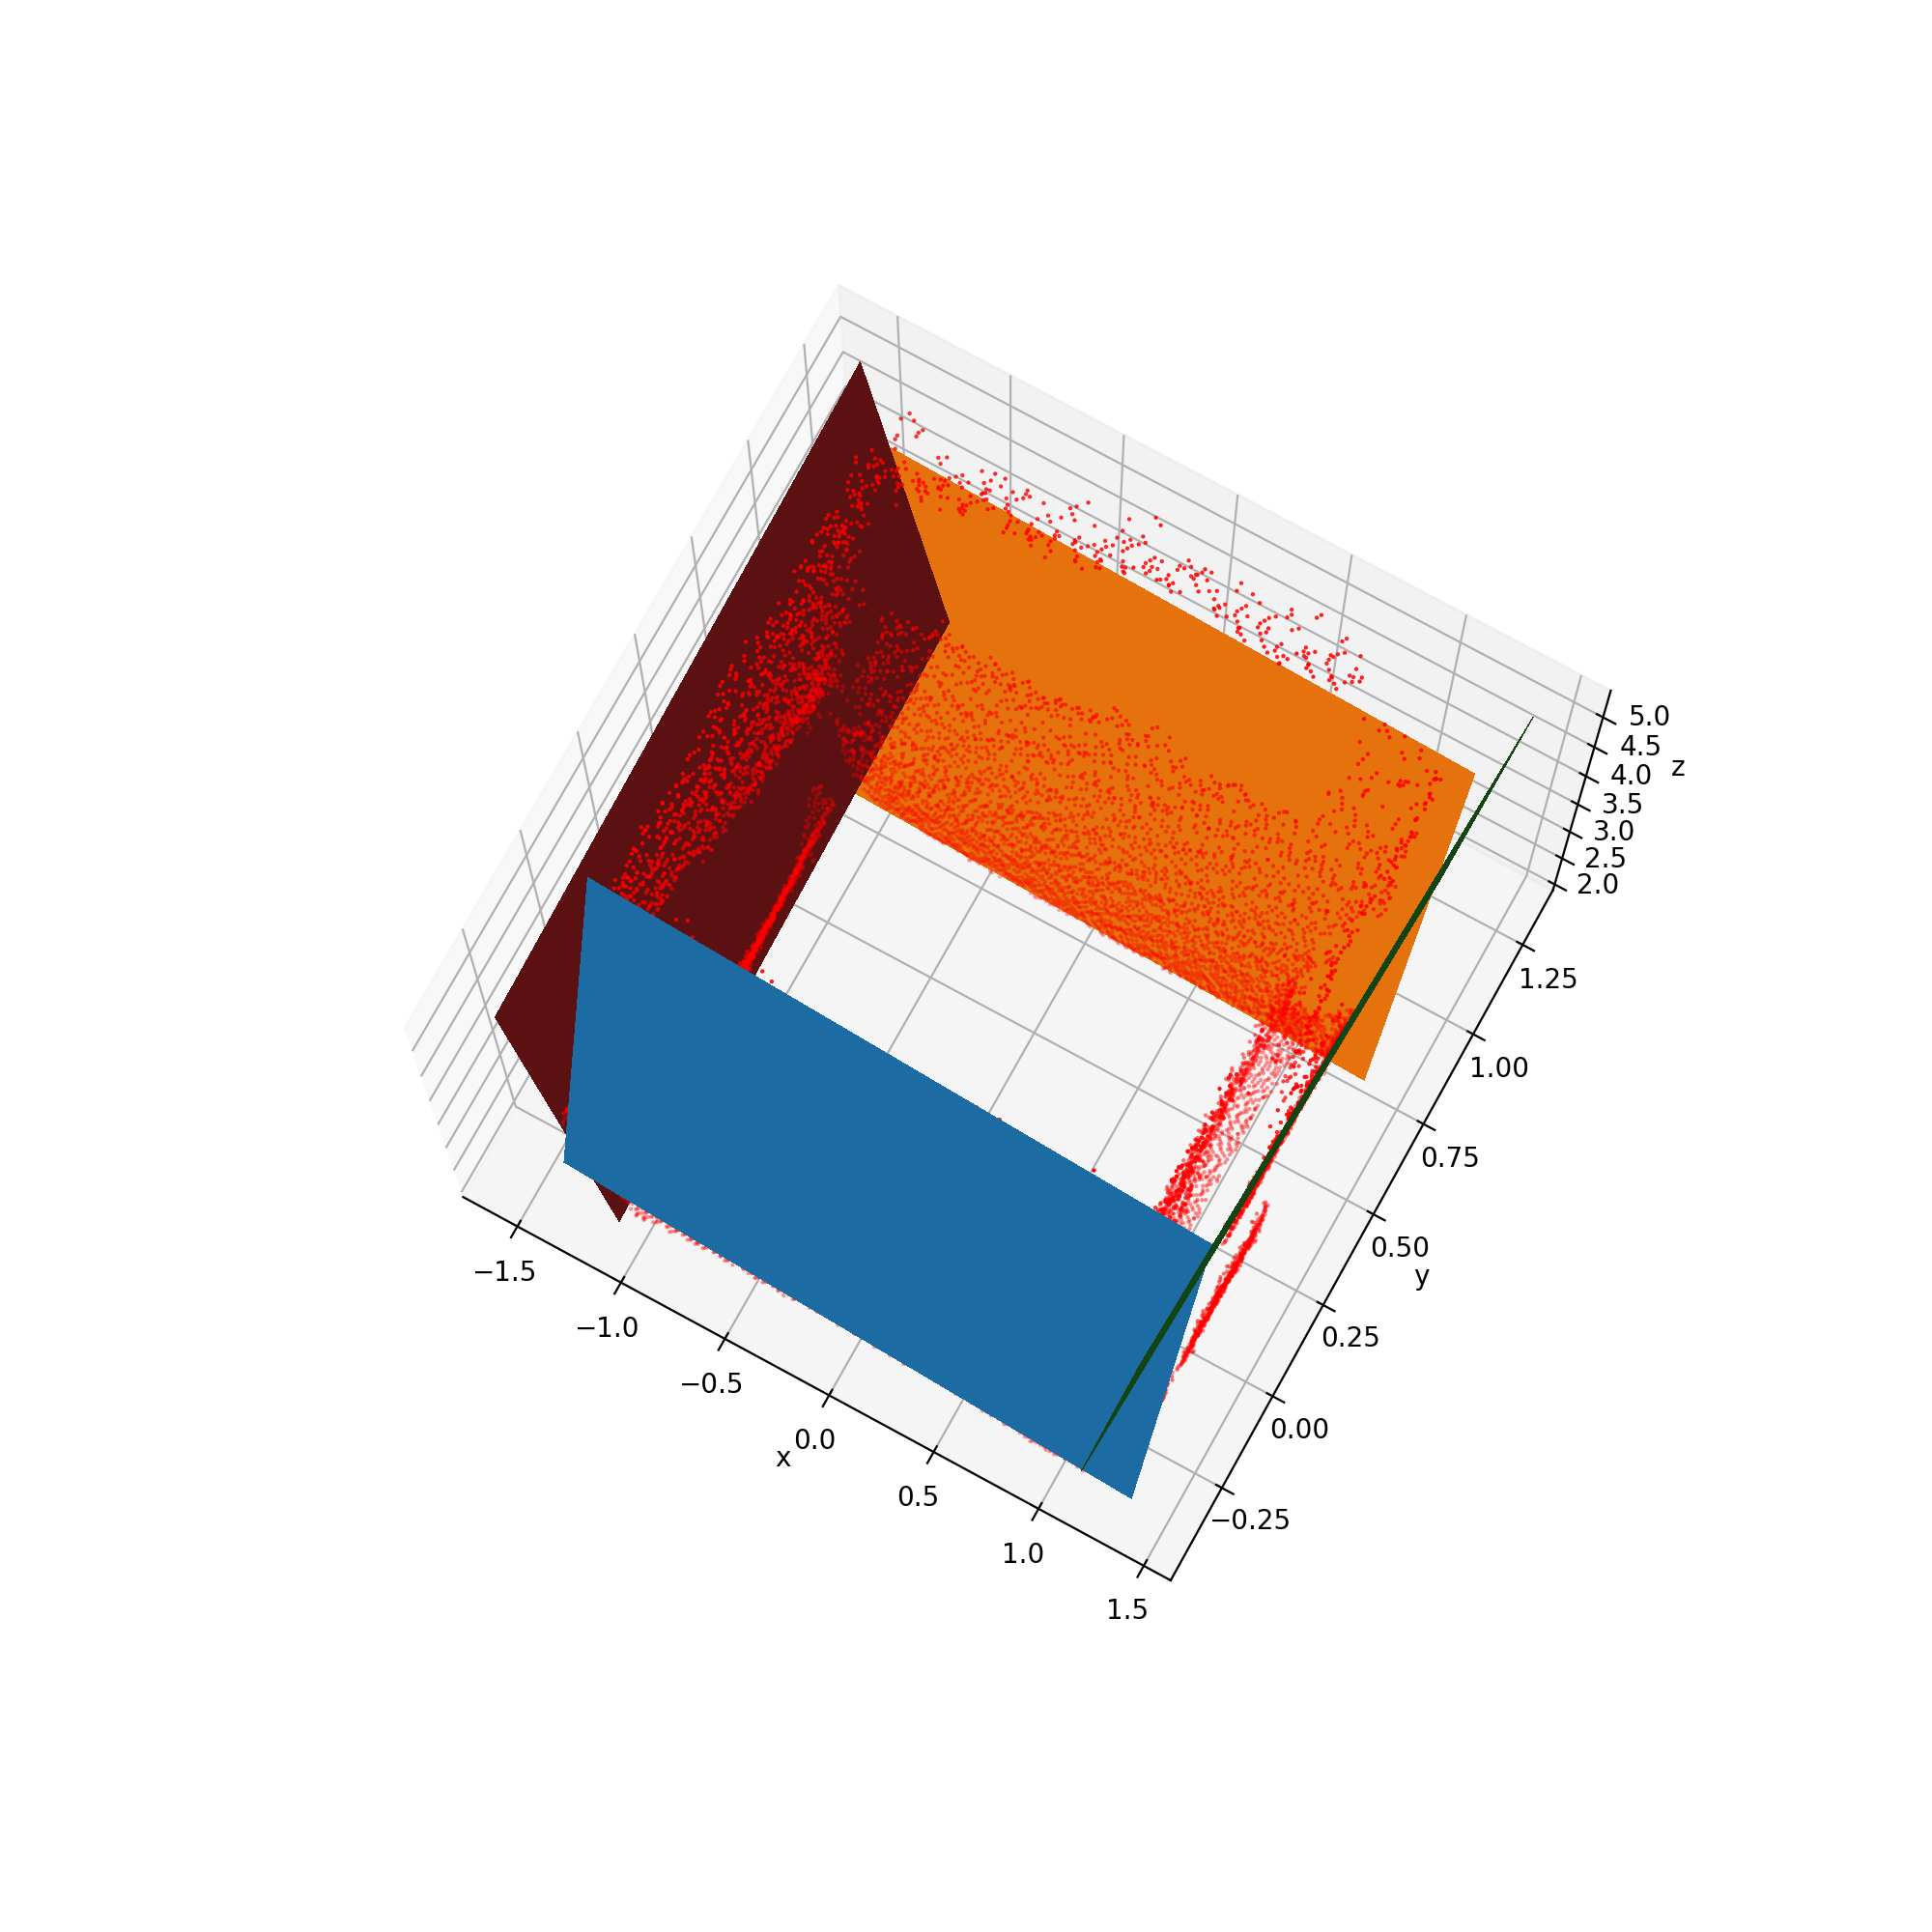
\includegraphics[width=\textwidth]{math/fig/hw3/ex4e.png}
    \caption{Ex4(e) Fitted plane and data points.}
    \label{fig:hw3_ex4e}
\end{figure}
\end{document}